
\chapter{The role of trust in knowledge based communities} % Main chapter title
\label{ChapterTrust}

Information and communications technologies (ICTs) have enabled faster and easier creation and sharing of knowledge. Furthermore, they have provided access to a large amount of data which enabled a detailed study of their emergence and evolution \cite{dankulov2015dynamics}, as well as user's roles \cite{saxena2021users}, patterns of their activity \cite{santos2019activity, slag2015one, chhabra2020activity}. 
However, relatively small attention was given to sustainability of SE communities. Most of the research was focused on the activity and factors that influence the increase of the users’ activity in these communities. Factors such as need for experts and the quality of their contributions have been thoroughly investigated \cite{dev2018size}. It was shown that growth of communities and mechanisms that drive it may depend on the topic around which the community was created \cite{santos2019self}.

The \textbf{Stack Exchange} is a network of question-answer websites on diverse topics. In the beginning, the focus was on computer programming questions with StackOverflow \footnote{
	More information about StackOverlflow is available at: \url{https://stackoverflow.co/} and broad introduction to StackExchange network is available at: \url{https://stackexchange.com/tour}. 
}  community. Its popularity led to the creation of the Stack Exchange network that these days counts more than 100 communities on different topics. The SE communities are self-moderating, and the questions and answers can be voted, allowing users to earn Stack Exchange reputation and privileges on the site. 

The new site topics are proposed through site Area51 \footnote{Visit \url{https://area51.stackexchange.com/faq} for more details about closed and beta SE communities and the review process.}, and if the community finds them relevant, they are created. Every proposed  StackExchange site needs interested users to commit to the community and contribute by posting questions, answers and comments. After a successful private beta phase site reaches the public beta phase, other members are allowed to join the community. The site can be in the public beta phase for a long time until it meets specific SE evaluation criteria for graduation. Otherwise, it may be closed with a decline in users' activity. 

We focused analysis on four pairs of SE communities with the same topic. Astronomy, Literature and Economics are active communities \footnote{Astronomy, Literature and Economics graduated on December 2021 and during our research, they were still in the public beta phase.} The first time, these communities were unsuccessful and thus closed. We also compare closed Theoretical Physics with the Physics site, considering that those two topics engage similar type of users.

\section{Network properties of Stack Exchange data}

On Stack Exchange sites, the interaction between users happens through posts. As we are interested in examining the characteristics of the users, we map interaction data to the networks. Using complex network theory, we can quantify the properties of obtained networks and compare different SE communities, e.g. alive and closed SE sites. 

In the user interaction network, the link between two nodes, user $i$ and $j$, exists if user $i$ answers or comments on the question posted by user $j$, or user $i$ comments on the answer posted by user $j$. The created network is undirected and unweighted, meaning that we do not consider multiply interactions between users or the direction of the interaction. 

First approach is to aggregate all interactions in the first 180 days, and study the properties of static network. Many local and global network measures are dependent 
\cite{boccaletti2006complex}, and it was shown that degree distribution, degree-degree correlations and clustering coefficient are sufficient for description of the properties of complex networks \cite{orsini2015quantifying}. 
 
 
We calculate the \textbf{degree distribution}, figure \ref{fig:fullnetdeg}, and compare the distributions of active and closed communities of the same topic. Degree distributions between active and closed communities follow similar lines. 
 
 \begin{figure}[h]
 	\centering
 	\includegraphics[width=\linewidth]{figures/stackexchange/degree_distribution_fullnet.pdf}
 	\caption{Degree distribution.}
 	\label{fig:fullnetdeg}
 \end{figure}
 
If we take look into \textbf{neighbor degree} dependece on the node degree $k_{nn}(k)$, figure \ref{fig:fullneighdeg} we find that there are structural differences between networks formed in the active and closed communities. On average $k$-degree users in active communities have neighbors with larger degree than it is case in closed communities. The results are consistent for Physics, Economics and Literature. For Astronomy we find different behavior, where the $k_{nn}(k)$ distributions of closed communities are on the top of distributions of the active one. 

\begin{figure}[h]
	\centering
	\includegraphics[width=\linewidth]{figures/stackexchange/neighdeg_fullnet.pdf}
	\caption{Neighbour degree.}
	\label{fig:fullneighdeg}
\end{figure}





The \textbf{clustering coefficient} of a node quantifies the average connectivity of between its neighbours and cohesion of its neighborhood \cite{boccaletti2006complex}. It is a probability that two neighbours of a node are also neighbours, and is calculated using the following formula:
\begin{equation}
c_{i}=\frac{e_{i}}{\frac{1}{2}k_{i}(k_{1}-1)} \ .
\label{eq:clust}
\end{equation}
Here $e_{i}$ is the number of links between neighbours of the node $i$ in a network, while $\frac{1}{2}k_{i}(k_{i}-1)$ is the maximal possible number of links determined by the node degree $k_{i}$. The clustering coefficient of network $C$ is the value of clustering averaged over all nodes. Study on dynamics of social group growth shows that that links between one's friends that are members of a social group increase the probability that that individual will join the social group \cite{backstrom2006group}. Furthermore, successful social diffusion  typically occur in networks with high value of clustering coefficient \cite{centola2007cascade}. These results suggest that high local cohesion should be a characteristic of sustainable communities. The dependence of the clustering coefficient on the node degree is shown on figure \ref{fig:fullclustering}. As expected we find that active communities are more clustered.

\begin{figure}[h]
	\centering
	\includegraphics[width=\linewidth]{figures/stackexchange/clustering_fullnet.pdf}
	\caption{Clustering coefficient.}
	\label{fig:fullclustering}
\end{figure}

\subsection{Properties of evolving complex networks}

Instead of creating a static network from the data in the first 180 days of community life, we study how network snapshots evolve. At each time step $t$, we create network snapshot $G(t, t+\tau)$, for time window of the length $\tau$. We fix the time window to $\tau=30$ days and slide it by $t=1$ day through time. Discussion of how the length of the sliding window influences the results is given in appendix A. Sliding the time window by one day, we can capture changes in the network structure daily, as two 30 days consecutive networks overlap significantly. 

Here we investigate how clustering coefficient in a SE community is changing with time by calculating its value for all network snapshots. We compare the behavior of clustering for active and closed communities on the same topic in order to better understand how cohesion of these communities is changing over time. Figure \ref{fig:clustering} shows the evolution of mean clustering coefficient for all eight communities. All communities that are still alive are clustered, with the value of mean clustering coefficient higher than 0.1. Physics, the only launched community, has the value of clustering coefficient above 0.2 for the first 180 days.

During larger part of the observed period, the clustering coefficient of an active community is higher compared to the clustering coefficient of its closed pair. If we compare active communities with their closed counterpart, the closed communities have higher value of the mean clustering coefficient in the early phase while later communities that are still active have higher values of clustering coefficient. These results suggest that all communities have relatively high local cohesiveness, and that lower values of clustering coefficient in the later phase of community life may be an indicator of its decline. 

\begin{figure}
	\centering
	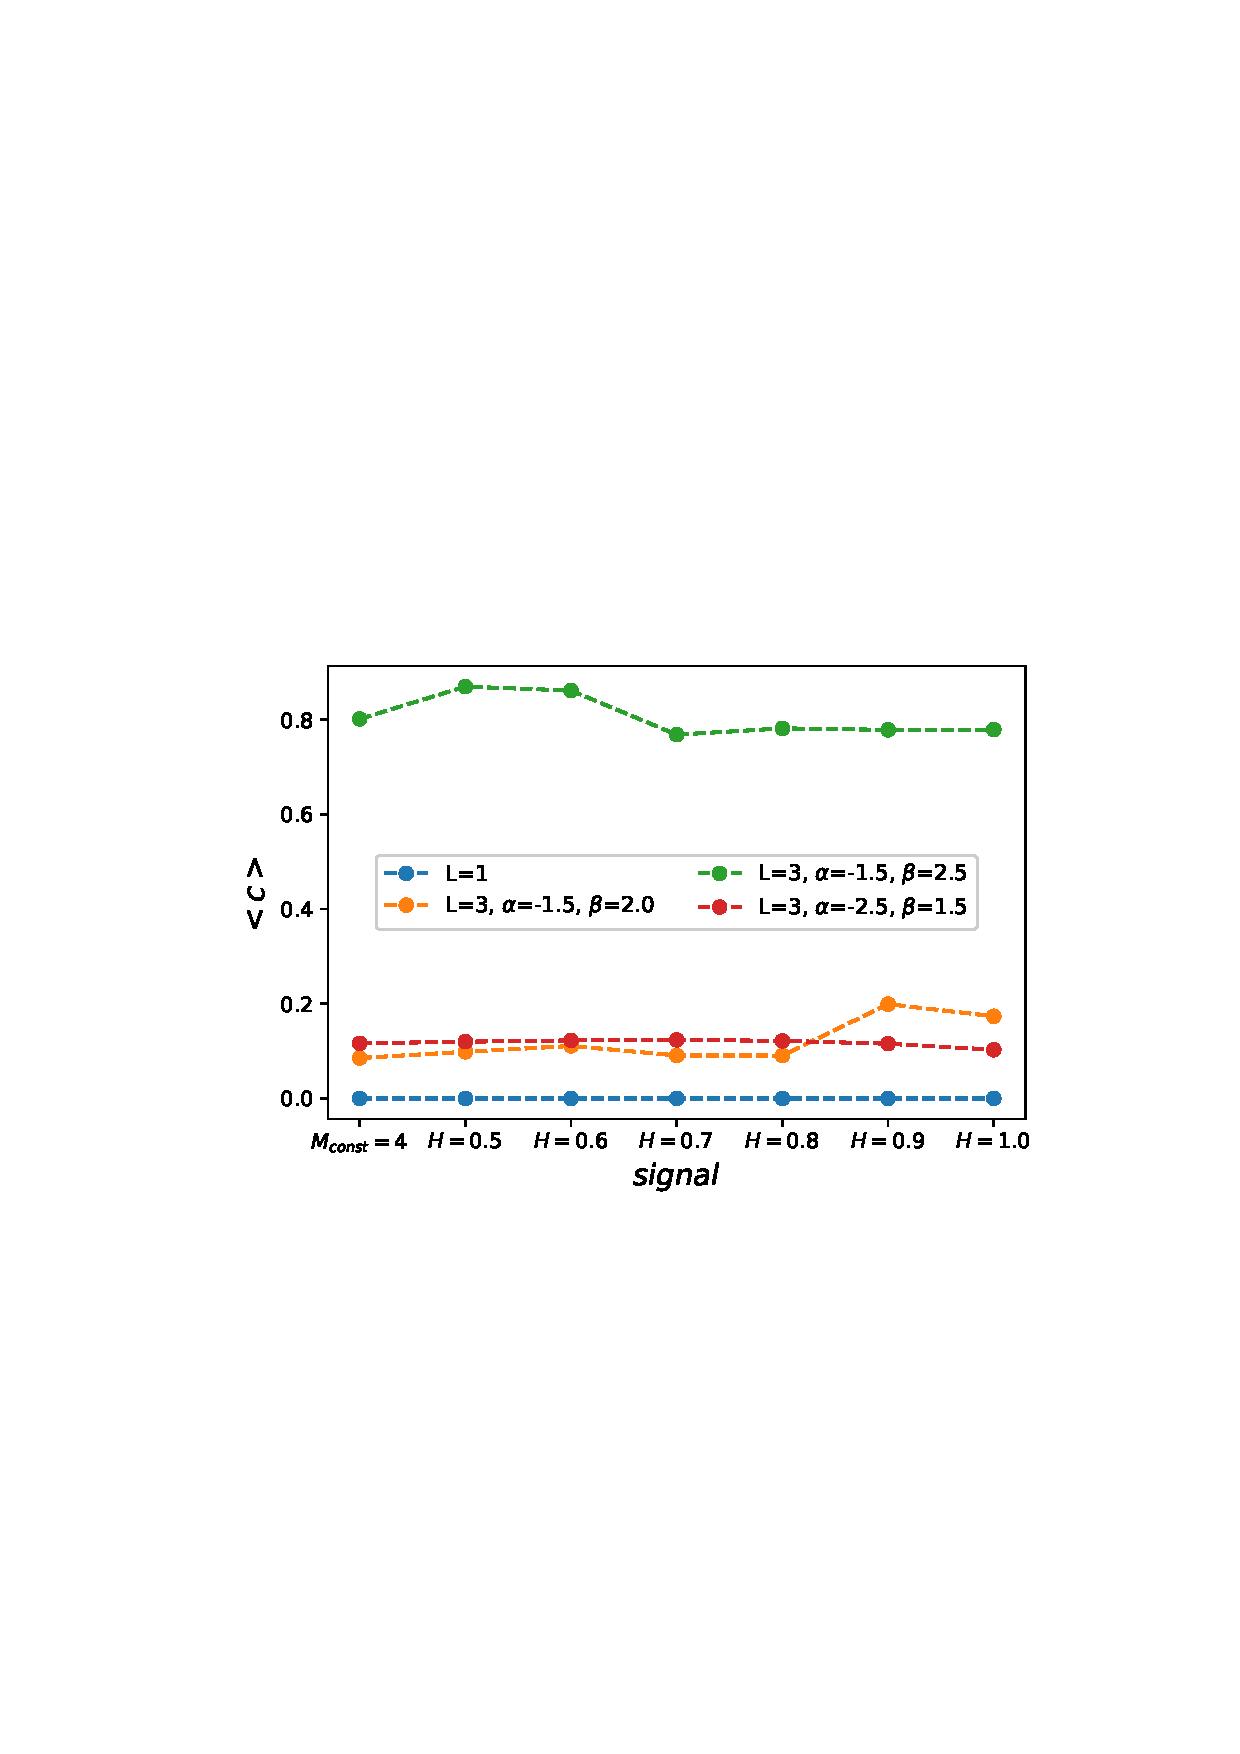
\includegraphics[width=\linewidth]{figures/stackexchange/clustering.pdf}%Figures/figures_SE/Fig3.pdf}
	\caption{Mean clustering coefficient.}
	\label{fig:clustering}
\end{figure}

